\PassOptionsToPackage{unicode=true}{hyperref} % options for packages loaded elsewhere
\PassOptionsToPackage{hyphens}{url}
\documentclass[11pt,dvipsnames,ignorenonframetext,aspectratio=169]{beamer}
\IfFileExists{pgfpages.sty}{\usepackage{pgfpages}}{}
\setbeamertemplate{caption}[numbered]
\setbeamertemplate{caption label separator}{: }
\setbeamercolor{caption name}{fg=normal text.fg}
\beamertemplatenavigationsymbolsempty
\usepackage{lmodern}
\usepackage{amssymb,amsmath}
\usepackage{ifxetex,ifluatex}
\usepackage{fixltx2e} % provides \textsubscript
\ifnum 0\ifxetex 1\fi\ifluatex 1\fi=0 % if pdftex
  \usepackage[T1]{fontenc}
  \usepackage[utf8]{inputenc}
\else % if luatex or xelatex
  \ifxetex
    \usepackage{mathspec}
  \else
    \usepackage{fontspec}
\fi
\defaultfontfeatures{Ligatures=TeX,Scale=MatchLowercase}







\fi

  \usetheme[]{monash}

  \usecolortheme{monashwhite}


% A default size of 24 is set in beamerthememonash.sty

% Title page
\setbeamertemplate{title page}
{\placefig{-0.01}{-0.01}{width=1.01\paperwidth,height=1.01\paperheight}{deepseashrimp.jpg}
\begin{textblock}{7.5}(1,2.8)\usebeamerfont{title}
{\color{white}\raggedright\par\inserttitle}
\end{textblock}
\begin{textblock}{7.5}(1,7)
{\color{white}\raggedright{\insertauthor}\mbox{}\\[0.2cm]
\insertdate}
\end{textblock}}


  \useinnertheme{rounded}

  \useoutertheme{smoothtree}

% use upquote if available, for straight quotes in verbatim environments
\IfFileExists{upquote.sty}{\usepackage{upquote}}{}
% use microtype if available
\IfFileExists{microtype.sty}{%
  \usepackage{microtype}
  \UseMicrotypeSet[protrusion]{basicmath} % disable protrusion for tt fonts
}{}


\newif\ifbibliography


\hypersetup{
      pdftitle={Path Analysis},
            colorlinks=true,
    linkcolor=red,
    citecolor=Blue,
    urlcolor=lightgrayd,
    breaklinks=true}
%\urlstyle{same}  % Use monospace font for urls







% Prevent slide breaks in the middle of a paragraph:
\widowpenalties 1 10000
\raggedbottom

  \AtBeginPart{
    \let\insertpartnumber\relax
    \let\partname\relax
    \frame{\partpage}
  }
  \AtBeginSection{
    \ifbibliography
    \else
      \let\insertsectionnumber\relax
      \let\sectionname\relax
      \frame{\sectionpage}
    \fi
  }
  \AtBeginSubsection{
    \let\insertsubsectionnumber\relax
    \let\subsectionname\relax
    \frame{\subsectionpage}
  }



\setlength{\parindent}{0pt}
\setlength{\parskip}{6pt plus 2pt minus 1pt}
\setlength{\emergencystretch}{3em}  % prevent overfull lines
\providecommand{\tightlist}{%
  \setlength{\itemsep}{0pt}\setlength{\parskip}{0pt}}

  \setcounter{secnumdepth}{0}


%% Monash overrides
\AtBeginSection[]{
   \frame<beamer>{
   \frametitle{Outline}\vspace*{0.2cm}
   
   \tableofcontents[currentsection,hideallsubsections]
  }}

% Redefine shaded environment if it exists (to ensure text is black)
\ifcsname Shaded\endcsname
  \definecolor{shadecolor}{RGB}{225,225,225}
  \renewenvironment{Shaded}{\color{black}\begin{snugshade}\color{black}}{\end{snugshade}}
\fi
%%

  \usepackage{setspace}
  \usepackage{wasysym}
  % \usepackage{footnote} % don't use this this breaks all
  \usepackage{fontenc}
  \usepackage{fontawesome}
  \usepackage{booktabs,siunitx}
  \usepackage{longtable}
  \usepackage{array}
  \usepackage{multirow}
  \usepackage{wrapfig}
  \usepackage{float}
  \usepackage{colortbl}
  \usepackage{pdflscape}
  \usepackage{tabu}
  \usepackage{threeparttable}
  \usepackage{threeparttablex}
  \usepackage[normalem]{ulem}
  \usepackage{makecell}
  \usepackage{xcolor}
  \usepackage{tikz} % required for image opacity change
  \usepackage[absolute,overlay]{textpos} % for text formatting
  \usepackage{chemfig}
  \usepackage[skip=0.333\baselineskip]{caption}
  % \newcommand*{\AlignChar}[1]{\makebox[1ex][c]{\ensuremath{\scriptstyle#1}}}%

  % this font option is amenable for beamer
  \setbeamerfont{caption}{size=\tiny}
  \singlespacing
  \definecolor{lightgrayd}{gray}{0.95}
  \definecolor{skyblued}{rgb}{0.65, 0.6, 0.94}
  \definecolor{oranged}{RGB}{245, 145, 200}

  % \newlength{\cslhangindent}
  % \setlength{\cslhangindent}{1.5em}
  % \newenvironment{cslreferences}%
  %   {\setlength{\parindent}{0pt}%
  %   \everypar{\setlength{\hangindent}{\cslhangindent}}\ignorespaces}%
  %   {\par}
    
  \newlength{\cslhangindent}
  \setlength{\cslhangindent}{1.5em}
  \newenvironment{CSLReferences}%
  {\setlength{\parindent}{0pt}%
  \everypar{\setlength{\hangindent}{\cslhangindent}}\ignorespaces}%
  {\par}

  \newcommand{\bcolumns}{\begin{columns}[T, onlytextwidth]}
  \newcommand{\ecolumns}{\end{columns}}

  \newcommand{\bdescription}{\begin{description}}
  \newcommand{\edescription}{\end{description}}

  \newcommand{\bitemize}{\begin{itemize}}
  \newcommand{\eitemize}{\end{itemize}}
  \AtBeginSubsection{}

  \title[]{Path Analysis}


  \author[
        Deependra Dhakal\\
Agriculture and Forestry University\\
\textit{ddhakal.rookie@gmail.com}\\
\url{https://rookie.rbind.io}
    ]{Deependra Dhakal\\
Agriculture and Forestry University\\
\textit{ddhakal.rookie@gmail.com}\\
\url{https://rookie.rbind.io}}


\date[
      
  ]{
    }

\begin{document}

% Hide progress bar and footline on titlepage
  \begin{frame}[plain]
  \titlepage
  \end{frame}


   \frame<beamer>{
   \frametitle{Outline}\vspace*{0.2cm}
   
   \tableofcontents[hideallsubsections]
  }

\hypertarget{introduction}{%
\section{Introduction}\label{introduction}}

\begin{frame}{}
\protect\hypertarget{section}{}
\begin{itemize}
\tightlist
\item
  Path analysis, alike the family of related regression models, is a
  linear model framework that models regression equations simultaneously
  with the given observed variables. It can be thought of as a special
  case of Structural Equation Modeling (SEM).
\item
  Variations of SEMs:

  \begin{itemize}
  \tightlist
  \item
    Simple regression
  \item
    Multiple regression
  \item
    Path analysis
  \item
    Confirmatory factor analysis
  \item
    Measurement model (Latent - Observed)
  \item
    Structural model (Latent - Latent)
  \end{itemize}
\end{itemize}
\end{frame}

\begin{frame}{}
\protect\hypertarget{section-1}{}
\begin{itemize}
\item
  The terminology of outcomes v.s. predictors breaks down when variables
  can be both outcomes and predictors at the same time.
\item
  It is normal to distinguish instead between:

  \begin{itemize}
  \tightlist
  \item
    Exogenous variables: those which are not predicted by any other
  \item
    Endogenous variables: variables which do have predictors, and may or
    may not predict other variables
  \end{itemize}
\item
  Path analysis is part of the set of techniques often termed
  `covariance modelling'. As the name implies the primary focus here is
  the relationships between variables, and less so the mean-structure of
  the variables.
\end{itemize}
\end{frame}

\begin{frame}{}
\protect\hypertarget{section-2}{}
\begin{itemize}
\tightlist
\item
  Path diagrams (common in SEM) are like flowcharts. They show variables
  interconnected with lines that are used to indicate causal flow.
\end{itemize}

\begin{figure}
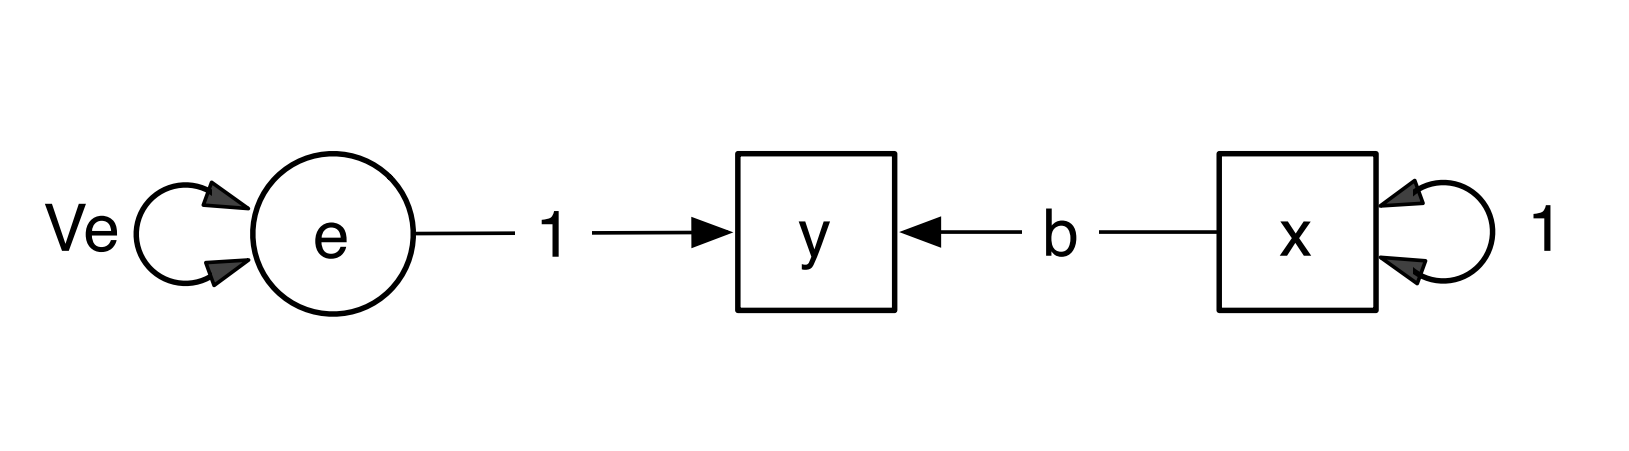
\includegraphics[width=0.8\linewidth]{../images/structural_equation} \caption{Such diagrams establish a simple isomorphism. All variables in the equation system are placed in the diagram, either in boxes or ovals. Each equation is represented on the diagram as follows: All independent variables (the variables on the right side of an equation) have arrows pointing to the dependent variable. The weighting coefficient is placed within the arrow. The above diagram shows a simple linear equation system and its path diagram representation.}\label{fig:simple-linear-path}
\end{figure}
\end{frame}

\begin{frame}{SEM modeling steps}
\protect\hypertarget{sem-modeling-steps}{}
\begin{itemize}
\tightlist
\item
  Statisticians have developed procedures for testing whether a set of
  variances and covariances in a covariance matrix fits a specified
  structure. The way structural modeling works is as follows:

  \begin{itemize}
  \tightlist
  \item
    You state the way that you believe the variables are inter-related,
    often with the use of a path diagram.
  \item
    You work out, via some complex internal rules, what the implications
    of this are for the variances and covariances of the variables.
  \item
    You test whether the variances and covariances fit this model of
    them.
  \item
    Results of the statistical testing, and also parameter estimates and
    standard errors for the numerical coefficients in the linear
    equations are reported.
  \item
    On the basis of this information, you decide whether the model seems
    like a good fit to your data.
  \end{itemize}
\end{itemize}
\end{frame}

\hypertarget{path-coefficients}{%
\section{Path coefficients}\label{path-coefficients}}

\begin{frame}{}
\protect\hypertarget{section-3}{}
\begin{itemize}
\tightlist
\item
  Path coefficients are standardized (Beta) or unstandardized (B or
  \(\beta\)) regression coefficients.
\item
  \textbf{Unstandardized} estimates of path coefficient retain scaling
  information of variables involved and can only be interpreted with
  reference to the scales of the variables.
\item
  \textbf{Standardized} estimates remove scaling information, and can be
  used for informal comparisons of parameters throughout the model; they
  correspond to effect size estimates.
\item
  Path coefficient (\(p_{DV,IV}\)) indicate the direct effect of IV to
  DV.
\item
  If the model contains only one IV and DV, the path coefficient equals
  to correlation coefficient.

  \begin{itemize}
  \tightlist
  \item
    In models that have more than two variables, the path coefficient
    equals to partial correlation coefficient.
  \item
    The other path coefficients are controlled while each individual
    path coefficient is calculated.
  \end{itemize}
\end{itemize}

\[SD = \large \sqrt{\frac{\sum (x-\bar{x})^2}{N-1}}; \large Z = \frac{(x - \bar{x})}{SD}\]
\end{frame}

\begin{frame}{}
\protect\hypertarget{section-4}{}
\begin{itemize}
\tightlist
\item
  Both unstandardized and standardized path coefficients are not
  correlation coefficients. Suppose we have a network with a path
  connecting from variable A to variable B.

  \begin{itemize}
  \tightlist
  \item
    with the unstandardized path coefficient B of 0.81, if variable A
    increases by one unit, variable B would be expected to increase by
    0.81 unit, while holding all other relevant variables constant.
  \item
    with the standardized path coefficient \(\beta\) of 0.81, if
    variable A increases by one standard deviation from its mean,
    variable B would be expected to increase by 0.81 its own standard
    deviations from its own mean while holding all other relevant
    variable constant.
  \end{itemize}
\end{itemize}
\end{frame}

\hypertarget{path-analysis-model-an-example}{%
\section{Path analysis model: An
example}\label{path-analysis-model-an-example}}

\begin{frame}{}
\protect\hypertarget{section-5}{}
\begin{table}

\caption{\label{tab:soydata-preview}A (fabricated) data showing variables having proposed roles in yield pathway.}
\centering
\fontsize{8}{10}\selectfont
\begin{tabular}[t]{lllllll}
\toprule
plants & pods\_plants & seeds\_pods & seed\_wt & pods\_branch & branch\_plant & grain\_yield\\
\midrule
14 & 102 & 2 & 75 & 9 & 11 & 1.1\\
14 & 92 & 2 & 62 & 10 & 10 & 1.01\\
18 & 83 & 3 & 86 & 6 & 14 & 1.44\\
... & ... & ... & ... & ... & ... & ...\\
15 & 72 & 2 & 76 & 6 & 9 & 1.17\\
\addlinespace
19 & 75 & 2 & 74 & 8 & 9 & 1.21\\
17 & 70 & 3 & 75 & 7 & 10 & 1.25\\
20 & 62 & 3 & 82 & 5 & 10 & 1.38\\
\bottomrule
\end{tabular}
\end{table}
\end{frame}

\begin{frame}{Conventions and symbology}
\protect\hypertarget{conventions-and-symbology}{}
\begin{itemize}
\item
  Circles are latent (unobserved) variables
\item
  Squares are manifest (observed) variables
\item
  Triangles can be used to interpret intercepts (part of square or
  circle but need to be turned on `specifically')
\item
  Except on specific model types (multigroup and latent growth), these
  are not estimated.
\end{itemize}
\end{frame}

\begin{frame}{}
\protect\hypertarget{section-6}{}
\begin{itemize}
\item
  Straight arrows are ``causal'' or directional
\item
  Non-standardized solution \(\longrightarrow\) these are the \(b\) or
  slope values
\item
  Standardized solution \(\longrightarrow\) these are beta values
  (standardized z score)
\item
  Curved arrows are non-directional
\item
  Non-standardized \(\longrightarrow\) covariance
\item
  Standardized \(\longrightarrow\) correlation
\item
  All endogenous variables (have arrows coming into them) have to have
  error terms.
\item
  Why is the arrow going into the variable ?

  \begin{itemize}
  \tightlist
  \item
    Because the error in the model is not explained by any other
    variable (otherwise it wouldn't be error).
  \end{itemize}
\end{itemize}
\end{frame}

\begin{frame}{Model fit}
\protect\hypertarget{model-fit}{}
\begin{itemize}
\tightlist
\item
  Model fits demonstrate which proposed model has the superior fit (how
  well the proposed theory fits the data).
\item
  Absolute fit index -- calculation does not rely on comparison with a
  baseline model
\item
  Absolute fit checks for SEMs:

  \begin{itemize}
  \tightlist
  \item
    \(\chi^2\) statistic
  \item
    RMSEA values (A cut-off value of RMSEA close to 0.06 (Hu and
    Bentler, 1999) or 0.07 (Steiger, 2007) seems to be the general
    consensus)
  \item
    Baseline model comparison
  \end{itemize}
\item
  Relative fit indices generally compare \(\chi^2\) value of a proposed
  model to a baseline model.
\end{itemize}
\end{frame}

\begin{frame}{}
\protect\hypertarget{section-7}{}
\includegraphics[width=0.85\linewidth]{06.3-path_analysis_files/figure-beamer/soybean-path-model-1}
\end{frame}

\hypertarget{assumptions-of-path-analysis-models}{%
\section{Assumptions of path analysis
models}\label{assumptions-of-path-analysis-models}}

\begin{frame}{Norm}
\protect\hypertarget{norm}{}
\begin{itemize}
\tightlist
\item
  In PA and SEM, the number of observations is not based on the sample
  size, but rather, on the number of variables in the model (k).

  \begin{itemize}
  \tightlist
  \item
    The specific formula for estimating number of observations:
    \(\frac{k(k+1)}{2}\)
  \end{itemize}
\item
  Degress of freedom (df) = \# observations - \# parameters
\item
  Model \textbf{identifiability}

  \begin{itemize}
  \tightlist
  \item
    If, df = 0 \(\longrightarrow\) just identified
  \item
    If, df \textgreater{} 0 \(\longrightarrow\) over identified
  \item
    If, df \textless{} 0 \(\longrightarrow\) under identified
  \end{itemize}
\item
  Path model is executable if df \(\geq\) 0.
\end{itemize}
\end{frame}

\begin{frame}{Assumptions}
\protect\hypertarget{assumptions}{}
\begin{itemize}
\item
  Because path analysis involves the solution of multiple linear
  regression equations, the dependent variables for all equations must
  be approximately normally distributed and the relationships among the
  variables are assumed to be causal, linear and additive. Logistic
  regression equations, implying multiplicative relationships, cannot be
  substituted. Other curvilinear relations or interactions are also
  prohibited.
\item
  Residuals are not correlated with the variables that predict the
  outcome variables toward which they point. This means that \(e\) is
  not correlated with variables \(X_1\) and \(X_2\). This assumption
  implies that all relevant variables are included in the model, and any
  unmeasured variables are not correlated with the specified predictor
  variables.
\end{itemize}

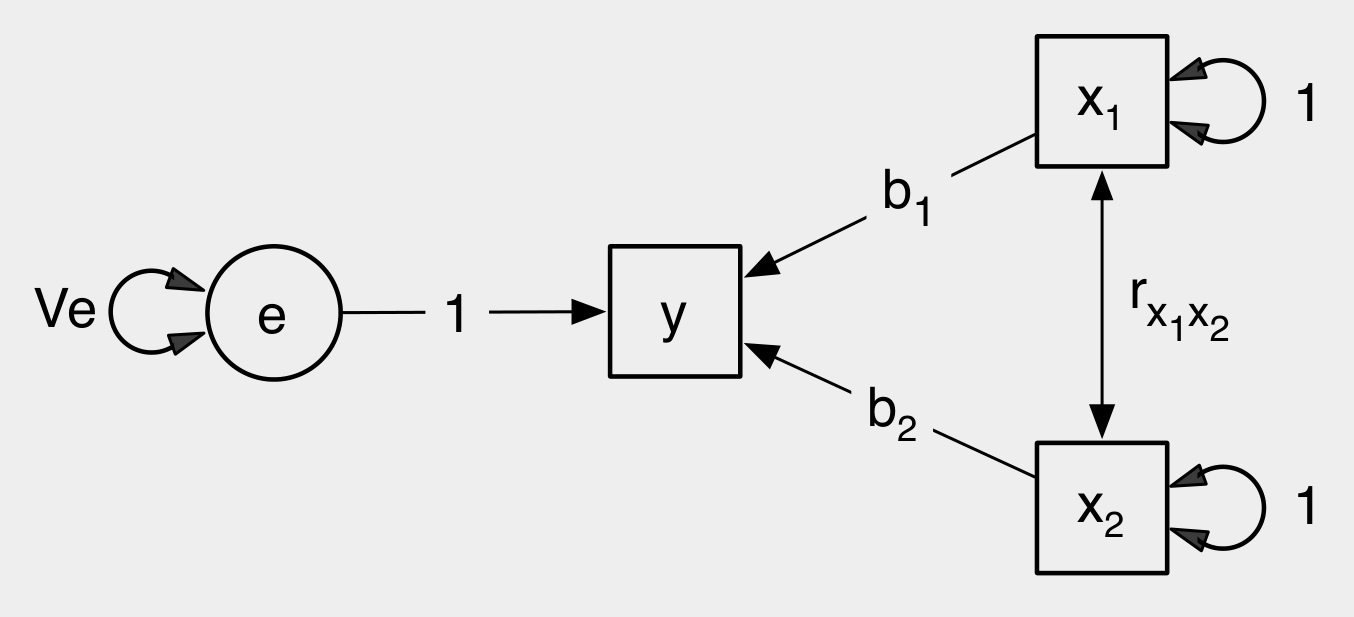
\includegraphics[width=0.8\linewidth]{../images/residual_independence}
\end{frame}

\begin{frame}{}
\protect\hypertarget{section-8}{}
\begin{itemize}
\item
  Causation flows in one direction; there are no feedback loops.
\item
  The variables are measured without error.
\item
  Predictor variables may be continuous, ordinal categorical, or
  dichotomous, but there may be no dummy variables.
\item
  There is low multicollinearity among predictor variables in any of the
  linear regression equations.
\end{itemize}
\end{frame}

\hypertarget{bibliography}{%
\section{Bibliography}\label{bibliography}}

\begin{frame}{References}
\protect\hypertarget{references}{}
\end{frame}




\end{document}
